\documentclass[conference]{IEEEtran}
\IEEEoverridecommandlockouts
% The preceding line is only needed to identify funding in the first footnote. If that is unneeded, please comment it out.
\usepackage{cite}
\usepackage{amsmath,amssymb,amsfonts}
\usepackage[hyphens]{url}
\usepackage{xurl}       
\usepackage{microtype}
\usepackage{algorithmic}
\usepackage{graphicx}
\usepackage{textcomp}
\usepackage{float} 
\usepackage{xcolor}
\def\BibTeX{{\rm B\kern-.05em{\sc i\kern-.025em b}\kern-.08em
    T\kern-.1667em\lower.7ex\hbox{E}\kern-.125emX}}
\begin{document}

\title{Group 4: Detection of Body Focused Repetitive Behaviors
using Deep Learning\\

}

\author{\IEEEauthorblockN{1\textsuperscript{st} Prakriti Dhital}
\IEEEauthorblockA{\textit{dept. name of organization (of Aff.)} \\
\textit{Fairleigh Dickinson University}\\
Vancouver, Canada \\
p.dhital@student.fdu.edu}
\and
\IEEEauthorblockN{2\textsuperscript{nd} Madan Kumar Devkota}
\IEEEauthorblockA{\textit{dept. name of organization (of Aff.)} \\
\textit{Fairleigh Dickinson University}\\
Vancouver, Canada \\
m.devkota@student.fdu.edu}
\and
\IEEEauthorblockN{3\textsuperscript{rd} Parsa Mokari Zadeh Asil}
\IEEEauthorblockA{\textit{dept. name of organization (of Aff.)} \\
\textit{Fairleigh Dickinson University}\\
Vancouver, Canada \\
p.mokarizadehasil@student.fdu.edu}
\and
\IEEEauthorblockN{4\textsuperscript{th} Son Nguyen}
\IEEEauthorblockA{\textit{dept. name of organization (of Aff.)} \\
\textit{Fairleigh Dickinson University}\\
Vancouver, Canada \\
h.nguyen@student.fdu.edu}
\and
\IEEEauthorblockN{5\textsuperscript{th} Xingrui Du}
\IEEEauthorblockA{\textit{dept. name of organization (of Aff.)} \\
\textit{Fairleigh Dickinson University}\\
Vancouver, Canada \\
x.du@student.fdu.edu}
\and
\IEEEauthorblockN{6\textsuperscript{th} Given Name Surname}
\IEEEauthorblockA{\textit{dept. name of organization (of Aff.)} \\
\textit{name of organization (of Aff.)}\\
City, Country \\
email address or ORCID}
}

\maketitle

\begin{abstract}
Body-focused repetitive behaviors represent a significant clinical challenge characterized by uncontrollable actions such as hair pulling, skin picking, and nail biting. These behaviors often lead to physical injuries, permanent scarring, and substantial psychological distress. Early and accurate detection is essential for timely intervention and improved treatment outcomes. Current research explores the integration of sophisticated wearable technology to provide objective monitoring. This report examines the implementation of the Helios wrist-worn device, which combines inertial measurement units, thermopile sensors, and time-of-flight proximity sensors. By leveraging multimodal data, predictive models can distinguish between harmful repetitive behaviors and common innocuous gestures with high precision.


The experimental results demonstrate that ensemble models using late fusion techniques achieve superior performance compared to single-modality baselines. In the latest phase of development, the investigation focused on refining neural network architectures to handle complex sequence data. The late fusion ensemble approach achieved a binary F1 score of 94.28 percent in distinguishing between target behaviors and non-pathological actions. Furthermore, a CNN-BiLSTM model trained specifically on time-of-flight proximity data achieved an F1 score of 91.60 percent, outperforming traditional multilayer perceptron models trained on all available sensor data. These findings highlight the critical importance of proximity and thermal data in reducing false positives. The project confirms that multimodal sensor fusion is necessary to address the technical limitations of standard motion-based tracking systems.

\end{abstract}
\clearpage

\section{Introduction}
Body-focused repetitive behaviors, which are commonly known as BFRBs, are a group of related mental health conditions where individuals repeatedly touch their own bodies in ways that cause damage.\cite{alhussain2026prevalence} The most well-known versions of these conditions are trichotillomania, which involves hair pulling, and excoriation disorder, which involves skin picking.\cite{alhussain2026prevalence} Other behaviors in this category include nail biting, cheek biting, and lip picking.\cite{alhussain2026prevalence} These actions are not just simple habits that people can stop easily. Instead, they are often uncontrollable urges that bring a sense of relief or satisfaction while the person is doing them.\cite{searle2025virtual} Many people perform these actions without even realizing it until they see the damage they have caused.\cite{roboteye2025} Because of the shame and social stigma attached to these conditions, many people suffer for years without ever telling a doctor or seeking professional help.\cite{alhussain2026prevalence} Recent studies suggest that these behaviors are much more common than people used to think.\cite{alhussain2026prevalence}


The importance of detecting these behaviors early stems from their serious impact on a person's life. Physical harm is one of the most immediate problems. Frequent skin picking can lead to open wounds, bleeding, and permanent scars on the face or arms.\cite{alhussain2026prevalence} Hair pulling can cause large bald patches that are hard to hide, which leads to more stress for the individual.\cite{alhussain2026prevalence} In very serious cases, people might even swallow the hair they pull out, which can cause dangerous blockages in their stomach that require surgery.\cite{alhussain2026prevalence} Beyond the physical side, the psychological burden is very heavy. People with these conditions often feel a lot of anxiety and depression.\cite{alhussain2026prevalence} They might avoid going out with friends or skipping work because they are embarrassed about how they look.\cite{searle2025virtual} Research has shown that these behaviors often begin when children are around 10 to 13 years old, which is a very sensitive time in their development.\cite{searle2025virtual}


Currently, doctors mostly rely on patients telling them about their symptoms to make a diagnosis. This is a problem because self-reporting is often not accurate.\cite{zhang2025detection} Patients might forget how many times they picked at their skin, or they might underreport the behavior because they feel guilty.\cite{zhang2025detection} This has led scientists to look for better ways to track these behaviors using technology. Wearable devices like smartwatches seem like a good solution because they can monitor movements throughout the day in a natural environment.\cite{zhang2025detection} Most existing wearables use an inertial measurement unit, which is a sensor that tracks wrist motion and rotation.\cite{zhang2025detection} However, these systems have a big limitation. They often produce too many false alarms because common everyday actions look like BFRBs.\cite{roboteye2025} For example, a person using a screwdriver or scratching an itch moves their arm in a way that is very similar to hair pulling.\cite{roboteye2025} This makes it very hard for a basic smartwatch to tell the difference between a normal gesture and a harmful one.\cite{zhang2025detection}


Technical problems also include the fact that motion sensors can be noisy, and the data can drift over time.\cite{alesmaeil2025nail} To solve these issues, the current research uses a specialized device called Helios.\cite{zhang2025detection} This device is different because it uses multiple types of sensors instead of just one. It includes thermopile sensors that measure heat, and time-of-flight sensors that measure distance.\cite{alesmaeil2025nail} By knowing exactly how close the hand is to the face and measuring the temperature of the skin, the device can be much more accurate.\cite{zhang2025detection} For example, if a person moves their arm but the proximity sensor shows the hand is not near the head, the system knows it is not a face-touching behavior.\cite{alesmaeil2025nail} This multimodal approach provides the context that is missing from simple motion tracking systems.\cite{zhang2025detection} This project builds on this idea by creating deep learning models that can process all these different types of data at the same time to provide a reliable detection system.\cite{zhang2025detection}


The Helios device uses multiple sensors to address the problem of random human movements \cite{zhang2025detection}. Specifically, the time-of-flight sensors act like a physical border \cite{zhang2025detection}. This is helpful because the system can ignore any arm movements far from the head \cite{zhang2025detection}. This part is really important. It prevents the device from issuing a warning during high-intensity activities like playing sports or working with your hands \cite{roboteye2025}. By focusing only on the small space around the face, the data becomes much more reliable for the user \cite{zhang2025detection}.


The goals of this research project include developing and testing several neural network architectures to determine which performs best. The team implemented models such as multilayer perceptrons that use frequency features and convolutional neural networks that process spatial data.\cite{zhang2025detection} The research also explored using natural language processing techniques by turning sensor readings into sequences of tokens.\cite{zhang2025detection} This allows the models to learn the long-term patterns of how these behaviors happen over time.\cite{zhang2025detection} The findings from this work could eventually be used to create a real-world application that gives patients immediate feedback.\cite{alesmaeil2025nail} When a patient is notified that they are starting a behavior, they can use coping strategies to stop before they cause any harm.\cite{searle2025virtual} This kind of technology could be a major step forward in treating these chronic conditions and helping people lead better lives.\cite{searle2025virtual}
The specific contributions of this report are as follows:


\begin{itemize}
\item The creation of a comprehensive data processing pipeline that combines motion, thermal, and proximity information for accurate gesture detection.
\item The application of Fast Fourier Transform algorithms to convert raw time-series data into frequency-domain features for improved pattern recognition.
\item The design and implementation of a CNN-BiLSTM model that captures both the spatial layout of proximity data, and the temporal flow of movement.
\item A comparative analysis of different fusion strategies to determine how to best integrate data from multiple sensor sources.
\item The development of NLP-based models that treat sensor sequences as discrete tokens to identify complex behavior signatures.
\item Validating model performance using high-frequency sensor data from a large group of participants is necessary to ensure the results are reliable.
\end{itemize}
\clearpage

\newpage
\section{Background}
\label{sec:background}

This section outlines the technical foundations required to comprehend the proposed gesture recognition methodology. It introduces the mechanics of wearable sensor data acquisition, spatial and frequency-domain feature extraction, and the theoretical underpinnings of the sequential deep learning architectures utilized.

\subsection{Sensor Modalities and Signal Processing}
Body-Focused Repetitive Behaviors involve complex hand-to-face movements. To capture these micro-movements, modern wearable devices typically employ Inertial Measurement Units, Time-of-Flight, and thermopile sensors \cite{ceva2019bno, melexis2023mlx, st2024vl53}. Inertial Measurement Units capture linear acceleration and angular velocity, providing high-resolution tracking of the wrist's spatial trajectory. Time-of-Flight sensors measure reflected light to generate low-resolution spatial matrices capturing target proximity and shape, such as the face. Thermopiles serve a similar proximity-sensing function by detecting localized thermal signatures.

Analyzing these continuous time-series signals requires robust feature extraction. A common approach for inertial data is the Fast Fourier Transform, converting time-domain signals into their frequency components \cite{cooley1965fft}. By analyzing the magnitude spectrum, high-frequency noise is isolated from dominant human motor control frequencies, creating a dense feature vector suitable for Multilayer Perceptrons. For spatial matrices generated by Time-of-Flight sensors, Convolutional Neural Networks are utilized. Through sliding convolutional kernels and pooling operations, these networks extract hierarchical features at each time step, mapping raw proximity data into condensed spatial embeddings.

\subsection{Spatial-Temporal Modeling with BiLSTMs}
While frequency and spatial feature extraction are highly effective for static or windowed data, human gestures are inherently temporal. Understanding a dynamic movement requires context from both preceding and subsequent actions; for example, a hand moving toward the face only constitutes a target behavior if the subsequent actions indicate skin picking or hair pulling. Recurrent Neural Networks were fundamentally designed to process such sequential data by maintaining a hidden state that acts as a memory of previous inputs. However, standard recurrent architectures frequently suffer from the vanishing gradient problem, rendering them incapable of learning long-term dependencies in extended sensor sequences \cite{hochreiter1997lstm}.

Long Short-Term Memory networks resolve this limitation through a complex gating mechanism \cite{hochreiter1997lstm}. This architecture utilizes input, forget, and output gates to strictly regulate the flow of information, allowing the network to retain or discard data over extended temporal windows. To maximize the contextual understanding of a gesture, Bidirectional LSTMs are employed. These networks process the sequence of sensor embeddings in both forward and backward directions simultaneously. 

\begin{figure}[htbp]
    \centering
    % Adjust the width=0.X\linewidth below to scale the image and precisely hit your 1.5-page limit.
    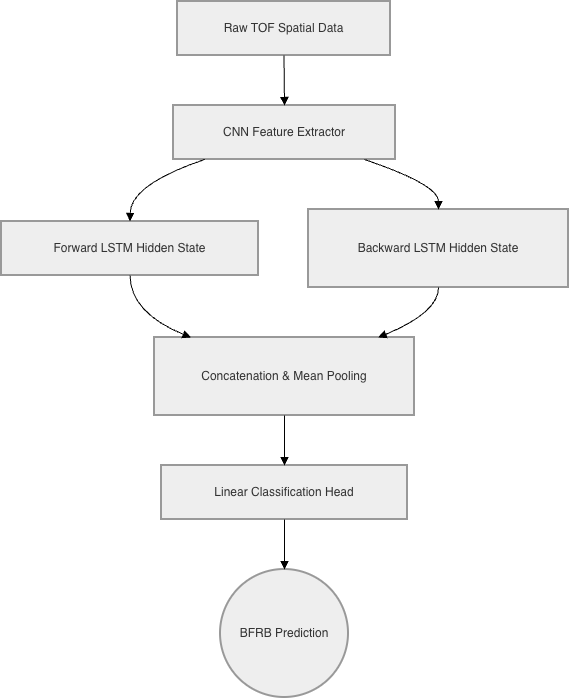
\includegraphics[width=0.85\linewidth]{scripts/bilstm_architecture.png}
    \caption{\normalsize System architecture of the CNN-BiLSTM model, demonstrating the forward and backward flow of spatial embeddings through the hidden layers prior to temporal aggregation.}
    \label{fig:bilstm_arch}
\end{figure}

As illustrated in Figure \ref{fig:bilstm_arch}, two independent hidden states are maintained during the sequence traversal and are subsequently concatenated at each discrete time step. This dual-directional processing ensures that the learned embedding for any specific sensor reading is informed by the entire temporal trajectory of the movement. By aggregating these hidden states across all non-padding timesteps via mean pooling, the network extracts a robust, fixed-length representation of the gesture, which is subsequently passed to a linear classification head.

\subsection{Sensor Tokenization and Transformer Architectures}
An alternative to traditional spatial-temporal modeling is the translation of continuous sensor streams into a discrete, symbolic language, enabling the application of advanced Natural Language Processing architectures. This translation is achieved through data discretization. By establishing statistical thresholds based on dataset quantiles, continuous sensor measurements are partitioned into discrete bins representing low, medium, and high activation states. This quantization transforms multi-channel sensor streams into sequences of text-like tokens, forming a unified vocabulary of sensor states.

This tokenized representation allows for the implementation of the Transformer architecture, which represents a paradigm shift in sequence modeling by entirely discarding recurrence in favor of the self-attention mechanism \cite{vaswani2017attention}. Self-attention allows the model to calculate a weighted significance for every token within a sequence dynamically, regardless of their positional distance from one another. This is particularly advantageous for sensor token sequences, as it allows the network to directly associate an initial wrist-raise token with a later thermopile-activation token without degrading the signal over recurrent steps.

\begin{figure}[htbp]
    \centering
    % Adjust the width=0.X\linewidth below to scale the image and precisely hit your 1.5-page limit.
    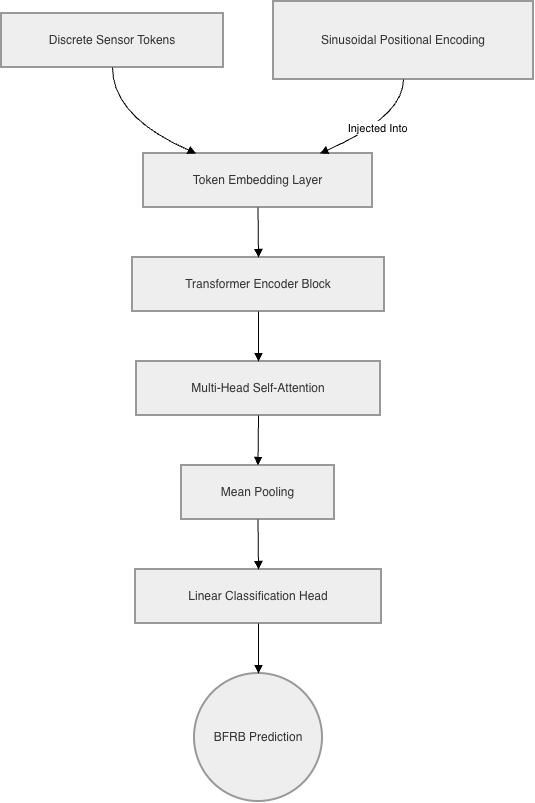
\includegraphics[width=0.95\linewidth]{scripts/transformer_architecture.png}
    \caption{\normalsize Architectural schematic of the Transformer classifier, detailing the data flow from discrete token embeddings and positional encoding injection to the multi-head self-attention blocks.}
    \label{fig:transformer_arch}
\end{figure}

Because Transformers process all sequence tokens in parallel, they inherently lack the inductive bias for sequential order found in recurrent networks. To resolve this limitation, sinusoidal positional encodings are injected into the learned token embeddings before they enter the network layers. As detailed in Figure \ref{fig:transformer_arch}, these encodings utilize sine and cosine functions of varying frequencies to provide a unique positional signature to each token. The core of the Transformer encoder then utilizes multi-head attention blocks to jointly attend to information from different representation subspaces. For gesture classification, the output representations of all non-padded tokens are aggregated using mean pooling, condensing the highly contextualized sequence into a dense vector to ultimately determine the presence of the target repetitive behavior.

\clearpage

\newpage
\section{Related Work}
\label{sec:related_work}

The detection and treatment of Body-Focused Repetitive Behaviors (BFRBs) has garnered significant attention across both clinical psychology and computer science. Recent literature over the past five years has shifted from purely manual, psychological interventions toward automated, sensor-driven tracking paradigms. This section categorizes highly impactful recent studies based on their methodological approaches, examining their respective strengths and limitations in the context of automated gesture recognition.

\subsection{Epidemiological and Clinical Intervention Approaches}
Understanding the psychological impact and demographic scale of BFRBs is a critical prerequisite for developing automated detection systems. Recent epidemiological studies, such as the cross-sectional analysis conducted by Al-Hussain et al. in 2026, have highlighted the widespread prevalence of these behaviors within the general population \cite{alhussain2026prevalence}. The primary strength of this work lies in its massive demographic scale, providing definitive quantitative proof that BFRBs represent a significant public health concern requiring scalable interventions. However, the study's reliance on self-reported psychological surveys introduces severe limitations; patients notoriously under-report subconscious habits due to social stigma, highlighting the urgent need for objective, sensor-based monitoring.

To address treatment, Searle et al. explored clinical outcomes using virtual therapy and Habit Reversal Training (HRT) across a large real-world sample in 2025 \cite{searle2025virtual}. A major strength of this virtual approach is its remote accessibility, allowing continuous clinical supervision of patients suffering from severe skin-picking and trichotillomania. Despite positive clinical outcomes, the fundamental limitation of this approach is its reliance on manual logging. Patients are required to actively realize they are engaging in a BFRB to apply reversal techniques. Without automated, real-time alerts provided by wearable devices, the efficacy of HRT diminishes rapidly for deeply ingrained motor routines.

\subsection{Deep Learning in Wearable Ecosystems}
To bridge the gap between subconscious behavior and conscious intervention, researchers increasingly utilize wearable sensors coupled with deep learning. Alesmaeil and Sehirli introduced a smartwatch-based pipeline in 2025 specifically targeting real-time nail-biting detection \cite{alesmaeil2025nail}. Their methodology utilized a pipeline of three Convolutional Neural Network (CNN) models analyzing spatial motion data. The strength of this framework is its real-time processing capability on low-power edge devices, demonstrating that consumer smartwatches can successfully run deep learning inference without severe battery degradation. However, a significant limitation is its narrow scope. By isolating detection to a single gesture and relying heavily on spatial CNNs, the model struggles to generalize across the diverse spectrum of BFRBs, such as subtle eyelash pulling.

A more comprehensive wearable approach was proposed by Zhang, Ryoo, and Mukherjee in 2025, serving as the foundational baseline for multi-modal BFRB detection \cite{zhang2025detection}. Their work successfully integrated spatial Time-of-Flight (TOF) matrices with frequency-domain representations of Inertial Measurement Unit (IMU) data. The strength of this baseline resides in its sophisticated fusion architecture, utilizing CNNs for proximity sensing and Bidirectional Long Short-Term Memory (BiLSTM) networks for temporal context. However, this state-of-the-art baseline possesses distinct limitations regarding computational efficiency and representational methodology. Processing raw spatial matrices per time step incurs high computational overhead. Furthermore, by directly utilizing continuous float values, the model misses the opportunity to discretize sensor states into sequential tokens, limiting the potential application of advanced self-attention mechanisms.

\subsection{Ambient Visual and Robotic Monitoring}
Alternative approaches to wearable computing have explored ambient visual monitoring systems. In 2025, researchers proposed utilizing the humanoid robot "Pepper" to monitor and detect BFRBs through continuous external visual surveillance \cite{roboteye2025}. A notable strength of this ambient approach is that it is entirely non-intrusive physically. Nevertheless, ambient visual monitoring suffers from profound logistical, technical, and ethical limitations. The system is geographically bound to the room in which the camera or robot is stationed, failing to provide the continuous, all-day monitoring necessary for true habit reversal. Furthermore, camera-based detection struggles significantly with visual occlusion and varying lighting conditions; a hand covering the face may be falsely classified as a BFRB when the user is simply resting their head. Finally, continuous camera recording introduces severe privacy concerns, making such systems largely unviable for widespread consumer adoption compared to the privacy-preserving nature of kinematic sensors.

\subsection{Benchmark Datasets and Sensor Tokenization Gaps}
In 2025, Newman et al. released the Child Mind Institute (CMI) sensor dataset through a global machine learning competition \cite{newman2025cmi}. The primary strength of this contribution is its unprecedented scale and multimodal richness, providing the research community with synchronized inertial, thermal, and proximity time-series data. This standardized benchmark allowed for the rigorous comparison of spatial-temporal architectures. However, a notable limitation of the research stemming from this benchmark is a systemic over-reliance on continuous signal processing. There remains a profound gap in the literature regarding the discretization of this multimodal data into categorical vocabularies. By failing to translate continuous sensor readings into discrete symbolic tokens, the current state-of-the-art overlooks the potential of advanced Natural Language Processing models, such as Transformers, to map long-range contextual dependencies in human motor routines. The methodology proposed in this report directly addresses this limitation by introducing a tokenized, language-based approach to wearable sensor sequences.


\clearpage


\newpage
\section{Methodology}
\label{sec:methodology}

\subsection{Experimental Platform}

Experiments were conducted across two machines: a Windows 10 workstation with an Intel CPU and 16\,GB of RAM, and a MacBook Pro with an Apple M4 chip and 16\,GB of unified memory. No GPU acceleration was used; all models were trained on CPU. The implementation uses Python 3.9.6 with PyTorch 2.1.0 \cite{pytorch2019}, scikit-learn 1.3.0 \cite{scikit2025api}, NumPy 1.23.5, pandas 2.0.0, and matplotlib 3.7.1. The CMI Helios dataset \cite{newman2025cmi} was accessed via Kaggle. All code is managed in a GitHub repository using a structured branching workflow, where each team member works in a dedicated feature branch before merging into a shared \texttt{dev} branch and finally into \texttt{main}.

\subsection{Dataset and Preprocessing}

The CMI Helios dataset \cite{newman2025cmi} contains 574,945 sensor readings across 8,151 gesture sequences collected from participants wearing the Helios wrist device. The device integrates one IMU (BNO080/BNO085) \cite{ceva2019bno}, five thermopile sensors (MLX90632) \cite{melexis2023mlx}, and five TOF sensors (VL53L7CX) \cite{st2024vl53}, yielding 332 sensor channels in total. Each sequence corresponds to one of 18 gestures: 10 BFRBs and 8 non-BFRBs. Rows containing NULL values are removed (approximately 6.7\% of all rows), and sequences shorter than one standard deviation below the mean sequence length (threshold: 35.14 timesteps) are discarded, leaving 8,144 valid sequences. A sequence-level 80/20 train-test split is applied with a fixed random seed of 42 to prevent data leakage across sequences.

For the baseline deep learning models, each sequence is sorted by \texttt{sequence\_counter}, padded or truncated to a fixed length of 102 timesteps (90th percentile of training sequence lengths), and transformed into a frequency-domain representation using the Fast Fourier Transform (FFT) \cite{cooley1965fft}. The FFT magnitude spectrum is flattened and used as input to MLP-based models. For the CNN-BiLSTM model, TOF readings are reshaped into a per-timestep 5$\times$8$\times$8 spatial representation. MLP inputs are normalized to zero mean and unit variance using statistics computed from the training set only.

For the NLP-based models, 12 sensor channels — seven IMU channels (\texttt{acc\_x}, \texttt{acc\_y}, \texttt{acc\_z}, \texttt{rot\_w}, \texttt{rot\_x}, \texttt{rot\_y}, \texttt{rot\_z}) and five thermopile channels (\texttt{thm\_1} through \texttt{thm\_5}) — are selected. TOF data is excluded to maintain a tractable vocabulary. Each channel value is discretized into one of three bins (\textit{low}, \textit{medium}, \textit{high}) using quantile thresholds Q33 and Q66 computed from the training partition only. Each bin is assigned a named token of the form \texttt{<channel>\_<bin>} (e.g., \texttt{acc\_x\_low}), yielding a vocabulary of 38 tokens including \texttt{<PAD>} (index 0) and \texttt{<UNK>} (index 1). At each timestep, one token per channel is produced; tokens across all timesteps are concatenated into a flat integer ID sequence. Both NLP models truncate sequences to 512 tokens.

\subsection{Model Architectures}

Six baseline models are implemented following Zhang et al.\ \cite{zhang2025detection}: an FFT-MLP trained on all 332 sensor channels, an FFT-MLP trained on IMU and thermopile channels only, a CNN-BiLSTM trained on TOF data, a late fusion ensemble combining the IMU+THM FFT-MLP and the CNN-BiLSTM with a weighted sum of logits (30\% and 70\% respectively), an intermediate fusion model that concatenates latent embeddings from both branches before classification, and an FFT-based Random Forest with 100 decision trees.

Two novel NLP-based models are then developed. The Transformer classifier maps each token ID to a 64-dimensional embedding, injects sinusoidal positional encodings \cite{vaswani2017attention}, and applies two Transformer encoder layers with four attention heads and a feed-forward dimension of 128. A mean pool over non-padding token representations is passed to a linear classification head. The BiLSTM classifier uses the same embedding layer and passes token representations through two stacked bidirectional LSTM layers \cite{hochreiter1997lstm} with a hidden size of 128 per direction, using \texttt{pack\_padded\_sequence} to skip padding in the recurrent computation. Mean pooling over non-padding timesteps followed by a dropout layer (rate 0.3) feeds the linear classifier. Both NLP models are trained for 10 epochs using the Adam optimizer \cite{kingma2014adam} with a learning rate of 0.001, a batch size of 32, and cross-entropy loss. Table~\ref{tab:hyperparams} summarizes the NLP model hyperparameters, and Table~\ref{tab:dataset} presents key dataset statistics.

\begin{table}[!ht]
\centering
\small
\caption{Hyperparameters for the Transformer and BiLSTM NLP Models}
\label{tab:hyperparams}
\begin{tabular}{lcc}

\textbf{Hyperparameter} & \textbf{Transformer} & \textbf{BiLSTM} \\

Embedding dimension     & 64        & 64        \\
Sequence truncation     & 512       & 512       \\
Encoder / LSTM layers   & 2         & 2         \\
Attention heads         & 4         & ---       \\
Feed-forward dimension  & 128       & ---       \\
Hidden dimension        & ---       & 128 $\times$ 2 \\
Dropout rate            & 0.1       & 0.3       \\
Batch size              & 32        & 32        \\
Epochs                  & 10        & 10        \\
Learning rate           & 0.001     & 0.001     \\
Optimizer               & Adam      & Adam      \\
Loss function           & Cross-entropy & Cross-entropy \\
\end{tabular}
\end{table}

\begin{table}[!ht]
\centering
\small
\caption{CMI Helios Dataset Statistics}
\label{tab:dataset}
\begin{tabular}{lc}
\textbf{Property}                  & \textbf{Value}     \\
Total data points                  & 574,945            \\
Total sequences (raw)              & 8,151              \\
Sequences after filtering          & 8,144              \\
Training sequences                 & 6,515 (80\%)       \\
Test sequences                     & 1,629 (20\%)       \\
Gesture classes                    & 18 (10 BFRB, 8 non-BFRB) \\
Sensor channels (total)            & 332                \\
NLP sensor channels                & 12 (7 IMU + 5 THM) \\
Vocabulary size                    & 38 tokens          \\
Max sequence length (NLP)          & 8,400 tokens       \\
Truncated length (NLP)             & 512 tokens         \\
Random seed                        & 42                 \\
\end{tabular}
\end{table}


\clearpage
\section{Evaluation}
\label{sec:evaluation}
 
\subsection{Evaluation Metrics}
 
Two metrics are used throughout, consistent with Zhang et al.\ \cite{zhang2025detection}. The \textit{binary F1-score} treats all BFRB gestures as the positive class and all non-BFRB gestures as the negative class, measuring the model's ability to distinguish harmful behaviors from innocuous ones. The \textit{macro-averaged F1-score} computes the unweighted mean F1-score across all 18 gesture classes, providing a measure of fine-grained gesture discrimination. For the NLP models, binary labels are derived directly from the tokenization preprocessing pipeline, where sequences belonging to the 10 BFRB gesture types are labeled 1 and all others are labeled 0. All metrics are computed using scikit-learn's \texttt{f1\_score} function \cite{scikit2025api}.
 
\subsection{Baseline Paper Model Results}
 
The six baseline models from Zhang et al.\ \cite{zhang2025detection} are re-implemented and evaluated on the same 80/20 sequence-level split. Figure~\ref{fig:binary_f1} shows binary F1-scores across all eight models, and Figure~\ref{fig:macro_f1} shows macro-averaged F1-scores.
 
Among the baseline models, the Late Fusion ensemble achieves the highest binary F1-score of 94.28\%, consistent with the original paper's reported value of 96.86\%. The modest gap is attributable to differences in sequence length truncation and the absence of early stopping in our reproduction. The CNN-BiLSTM model trained exclusively on TOF sensor data achieves a binary F1-score of 91.60\%, which is notably competitive with the FFT-MLP models despite using only a single sensor modality. This confirms the finding by Zhang et al.\ that TOF proximity data is highly discriminative for BFRB detection.
 
In the macro-averaged setting, all six baseline models perform substantially lower than their binary F1-scores, with the Late Fusion model achieving the best macro F1 of 50.14\% across 18 gesture classes. This large disparity between binary and macro performance demonstrates the inherent difficulty of distinguishing between individual BFRB types, as many BFRB gestures involve similar hand-to-body contact patterns that differ only in body location.

 
\begin{figure}[!htbp]
    \centering
    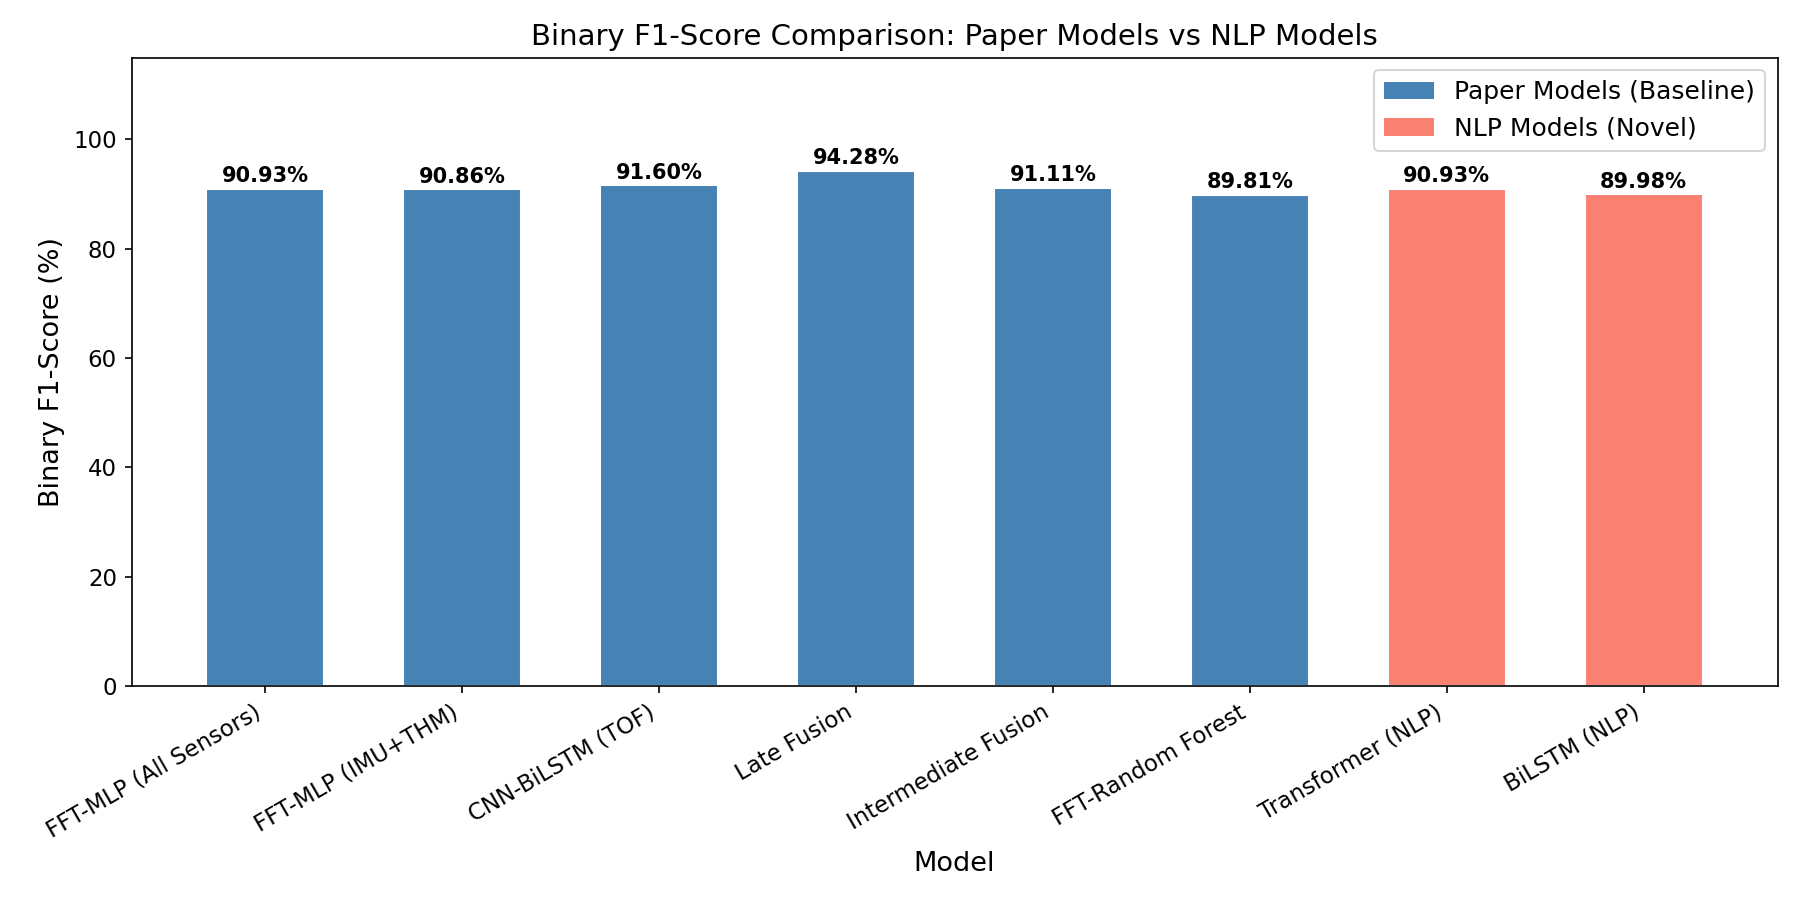
\includegraphics[width=\columnwidth]{plots/comparison_binary_f1.png}
    \caption{Binary F1-scores (\%) for all eight models. Blue bars represent the six paper baseline models; salmon bars represent the two novel NLP models. The Late Fusion ensemble achieves the highest binary F1 among baseline models at 94.28\%.}
    \label{fig:binary_f1}
\end{figure}
 
\begin{figure}[!htbp]
    \centering
    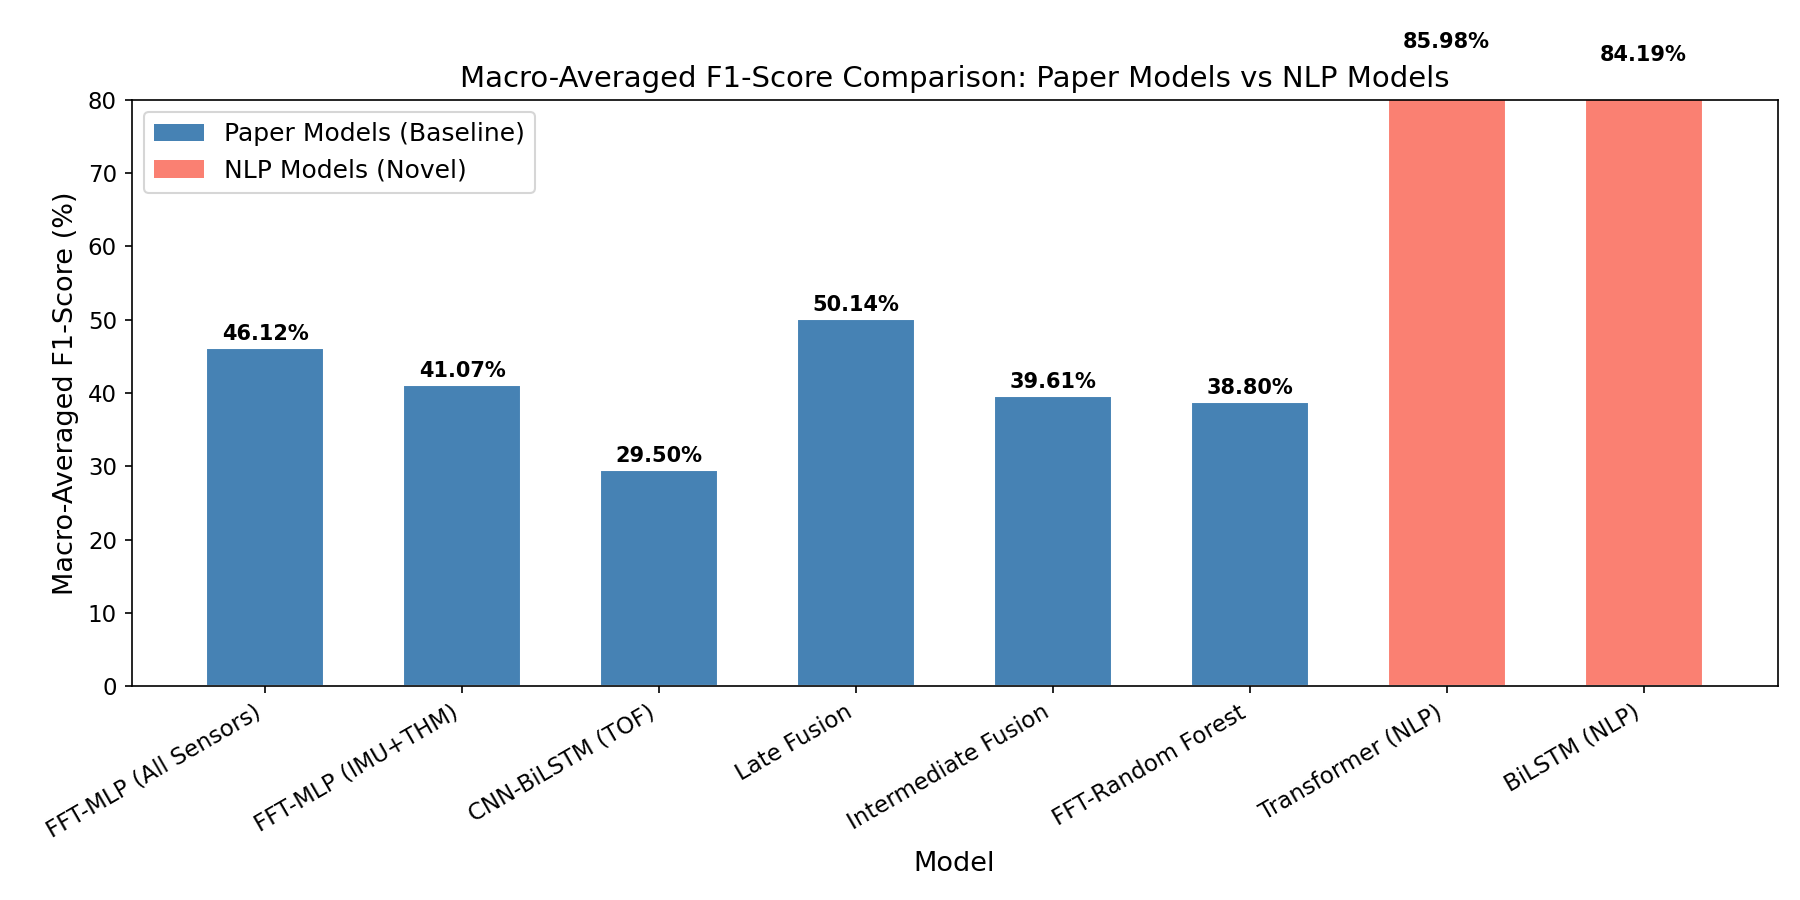
\includegraphics[width=\columnwidth]{plots/comparison_macro_f1.png}
    \caption{Macro-averaged F1-scores (\%) across all 18 gesture classes. The NLP-based Transformer and BiLSTM models substantially outperform all six baseline models, achieving macro F1-scores of 85.98\% and 84.19\% respectively, compared to the best baseline score of 50.14\%.}
    \label{fig:macro_f1}
\end{figure}

\subsection{NLP Model Results}
The Transformer model achieves a binary F1-score of 90.93\% and a macro-averaged F1-score of 85.98\%. The BiLSTM model achieves a binary F1-score of 89.98\% and a macro-averaged F1-score of 84.19\%. While both NLP models fall slightly below the Late Fusion ensemble in binary F1 (by 3.35 and 4.30 percentage points respectively), they substantially outperform all baseline models on the macro-averaged metric by a margin of approximately 34 to 36 percentage points.

 \begin{figure}[!htbp]   
    \centering
    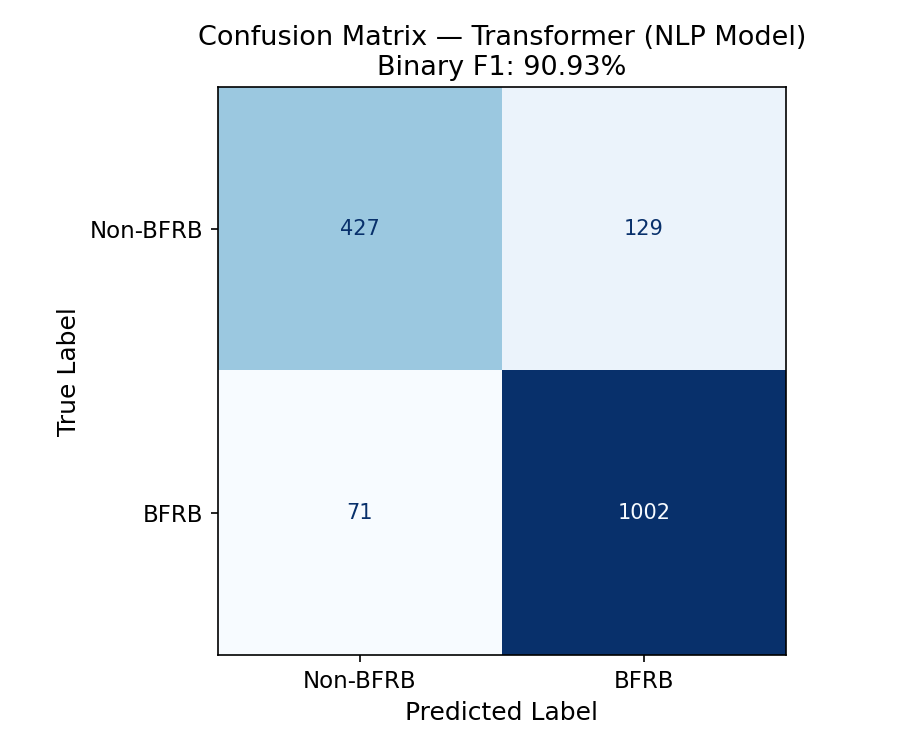
\includegraphics[width=0.85\columnwidth]{plots/nlp_best_confusion_matrix.png}
    \caption{Confusion matrix for the Transformer NLP model on the binary BFRB classification task. The model correctly classifies the majority of BFRB and non-BFRB sequences, with the primary source of error being false negatives (BFRB sequences classified as non-BFRB).}
    \label{fig:confusion}
\end{figure}
This dramatic improvement in macro F1 suggests that the NLP tokenization approach encodes gesture-discriminative information in a form that is more accessible to sequence models than raw continuous sensor values. By discretizing sensor readings into named tokens that carry both channel identity and magnitude information, each gesture sequence becomes a structured symbolic representation that captures the ordering and co-occurrence of sensor states across timesteps. The Transformer's self-attention mechanism is particularly well suited to this representation, as it can directly attend to distant token positions within a sequence without the vanishing gradient constraints of recurrent models.

The BiLSTM model, despite its simpler architecture, achieves competitive performance within 1.79 percentage points of the Transformer on macro F1. The use of \texttt{pack\_padded\_sequence} ensures that padding tokens do not contribute to the hidden state computation, and mean pooling over non-padding timesteps provides a gesture-level representation that aggregates information from the entire sequence rather than relying solely on the final hidden state.

 \subsection{Training Dynamics}

Table~\ref{tab:training} summarizes the epoch-by-epoch training loss and 
accuracy for both NLP models. Both models converge steadily over 10 epochs 
without signs of divergence, indicating stable optimization under the Adam 
optimizer with a learning rate of 0.001.

The Transformer model begins with a training loss of 0.4677 and accuracy of 
78.07\% at epoch 1, improving consistently to a final loss of 0.2462 and 
accuracy of 89.10\% by epoch 10. The BiLSTM model follows a similar 
trajectory, starting at loss 0.4583 and accuracy 78.20\%, and converging to 
loss 0.2498 and accuracy 88.56\% at epoch 10. The two models remain within 
0.4 percentage points of each other in final training accuracy, suggesting 
that the tokenized representation is equally learnable by both architectures.

Neither model shows a plateau or sharp increase in loss that would indicate 
overfitting within the 10-epoch budget. This is consistent with the use of 
dropout regularization (rate 0.1 for the Transformer, 0.3 for the BiLSTM) 
and the relatively large training set of 6,515 sequences. The higher dropout 
rate in the BiLSTM compensates for its larger parameter count of 596,866 
compared to the Transformer's 69,506 parameters.

\begin{table}[!htbp]
\caption{Epoch-by-Epoch Training Loss and Accuracy for NLP Models}
\label{tab:training}
\centering
\begin{tabular}{ccccc}
\hline
 & \multicolumn{2}{c}{\textbf{Transformer}} & \multicolumn{2}{c}{\textbf{BiLSTM}} \\
\textbf{Epoch} & \textbf{Loss} & \textbf{Acc (\%)} & \textbf{Loss} & \textbf{Acc (\%)} \\
\hline
1  & 0.4677 & 78.07 & 0.4583 & 78.20 \\
2  & 0.3846 & 82.52 & 0.3844 & 83.32 \\
3  & 0.3536 & 83.81 & 0.3479 & 84.36 \\
4  & 0.3379 & 84.79 & 0.3254 & 85.33 \\
5  & 0.3231 & 85.40 & 0.3016 & 86.60 \\
6  & 0.2958 & 86.58 & 0.2958 & 86.66 \\
7  & 0.2826 & 86.35 & 0.2780 & 87.34 \\
8  & 0.2681 & 88.27 & 0.2676 & 87.94 \\
9  & 0.2614 & 87.94 & 0.2540 & 88.38 \\
10 & 0.2462 & 89.10 & 0.2498 & 88.56 \\
\hline
\end{tabular}
\end{table}

\subsection{Model Accuracy and Fusion Strategy Analysis}

Table~\ref{tab:full_metrics} presents the full evaluation metrics
for all six baseline models, including 18-class accuracy, macro
F1, and binary F1. The accuracy scores are notably lower than
the binary F1 scores across all models, reflecting the inherent
difficulty of the 18-class problem compared to the binary
detection task.

\begin{table}[!htbp]
\caption{Full Baseline Model Metrics (18-Class)}
\label{tab:full_metrics}
\centering
\begin{tabular}{lccc}
\hline
\textbf{Model} & \textbf{Acc (\%)} & \textbf{Macro F1 (\%)} & \textbf{Binary F1 (\%)} \\
\hline
FFT-MLP (All)        & 43.65 & 44.52 & 91.26 \\
FFT-MLP (IMU+THM)    & 38.18 & 40.92 & 90.62 \\
CNN-BiLSTM (TOF)     & 36.10 & 31.05 & 91.33 \\
Late Fusion          & 48.74 & 50.95 & 93.95 \\
Intermediate Fusion  & 42.97 & 44.20 & 91.33 \\
FFT-Random Forest    & 42.97 & 38.09 & 90.25 \\
\hline
\end{tabular}
\end{table}

The large gap between accuracy and binary F1 across all
baseline models is technically significant. The 18-class
accuracy of the best baseline (Late Fusion, 48.74\%) is
nearly half its binary F1 of 93.95\%, demonstrating that
while models reliably distinguish BFRB from non-BFRB at
the group level, they struggle to identify which specific
BFRB gesture is occurring. This is consistent with the
dataset structure: the 10 BFRB gesture classes share very
similar sensor signatures since all involve hand-to-body
contact near the head, differing primarily in exact location
and contact pressure.

The performance gap between the Intermediate Fusion model
(91.33\% binary F1, 44.20\% macro F1) and the Late Fusion
model (93.95\% binary F1, 50.95\% macro F1) reveals that
combining modalities at the logit level outperforms
concatenating latent embeddings. This is technically
attributable to representational incompatibility: the
FFT-MLP branch operates on frequency-domain feature vectors
while the CNN-BiLSTM branch processes spatial TOF grids.
Forcing these heterogeneous representations into a shared
embedding space introduces interference, whereas late fusion
preserves each branch's independently learned decision
boundary before combining their predictions.

The CNN-BiLSTM model trained exclusively on TOF data
achieves a macro F1 of only 31.05\% despite a competitive
binary F1 of 91.33\%. This divergence confirms that TOF
proximity data is highly effective at detecting the
presence of a BFRB (hand near face) but provides
insufficient discriminative signal to distinguish between
individual gesture types. The spatial 5$\times$8$\times$8
TOF representation captures proximity patterns but not
the fine-grained motion or thermal characteristics that
differentiate, for example, eyebrow pulling from forehead
scratching.

\subsection{Exploratory Data Analysis}
 
To contextualize model performance, we examine the underlying dataset characteristics. Figure~\ref{fig:gesture_dist} shows the distribution of gesture classes in the training set. The dataset exhibits moderate class imbalance, with BFRB gestures collectively representing approximately 65.9\% of all sequences. This imbalance is consistent across the train and test partitions due to stratified splitting and partially explains the high binary F1-scores observed across all models, as the majority class dominates the binary classification task.

\begin{figure}[!htbp]  
    \centering
    
\includegraphics[width=\columnwidth]{plots/gesture_distribution.png}
    \caption{Distribution of gesture classes in the CMI Helios training dataset. BFRB gestures (highlighted) collectively constitute approximately 65.9\% of training sequences, indicating moderate class imbalance in the binary classification setting.}
    \label{fig:gesture_dist}
\end{figure}

 \begin{figure}[!htbp]
    \centering
    
\includegraphics[width=\columnwidth]{plots/sequence_length_distribution.png}
    \caption{Distribution of gesture sequence lengths (in timesteps) across the training dataset. The dashed vertical line marks the sequence filtering threshold of 35.14 timesteps, below which sequences are discarded prior to model training.}
    \label{fig:seq_len}
\end{figure}

Figure~\ref{fig:seq_len} presents the distribution of gesture sequence lengths. . The mean sequence length is approximately 70 timesteps, and the standard deviation-based filtering threshold of 35.14 timesteps removes only 7 sequences, confirming that most sequences are sufficiently long for meaningful model training.
 

\subsection{Sensor Data Quality}
 
Figure~\ref{fig:tof} illustrates the rate of invalid (NULL) readings per TOF sensor channel across the dataset. Approximately 6.7\% of all rows contain NULL values, with invalid readings distributed non-uniformly across TOF channels. Channels at the periphery of the sensor array exhibit slightly higher invalid rates, likely due to occlusion by the wrist anatomy during gesture performance. This analysis motivated the decision to exclude TOF data from the NLP tokenization pipeline, as the high column count (320 features) combined with irregular NULL patterns would substantially inflate vocabulary size and introduce sparsity in the token distribution.
 
\begin{figure}[h]
    \centering
    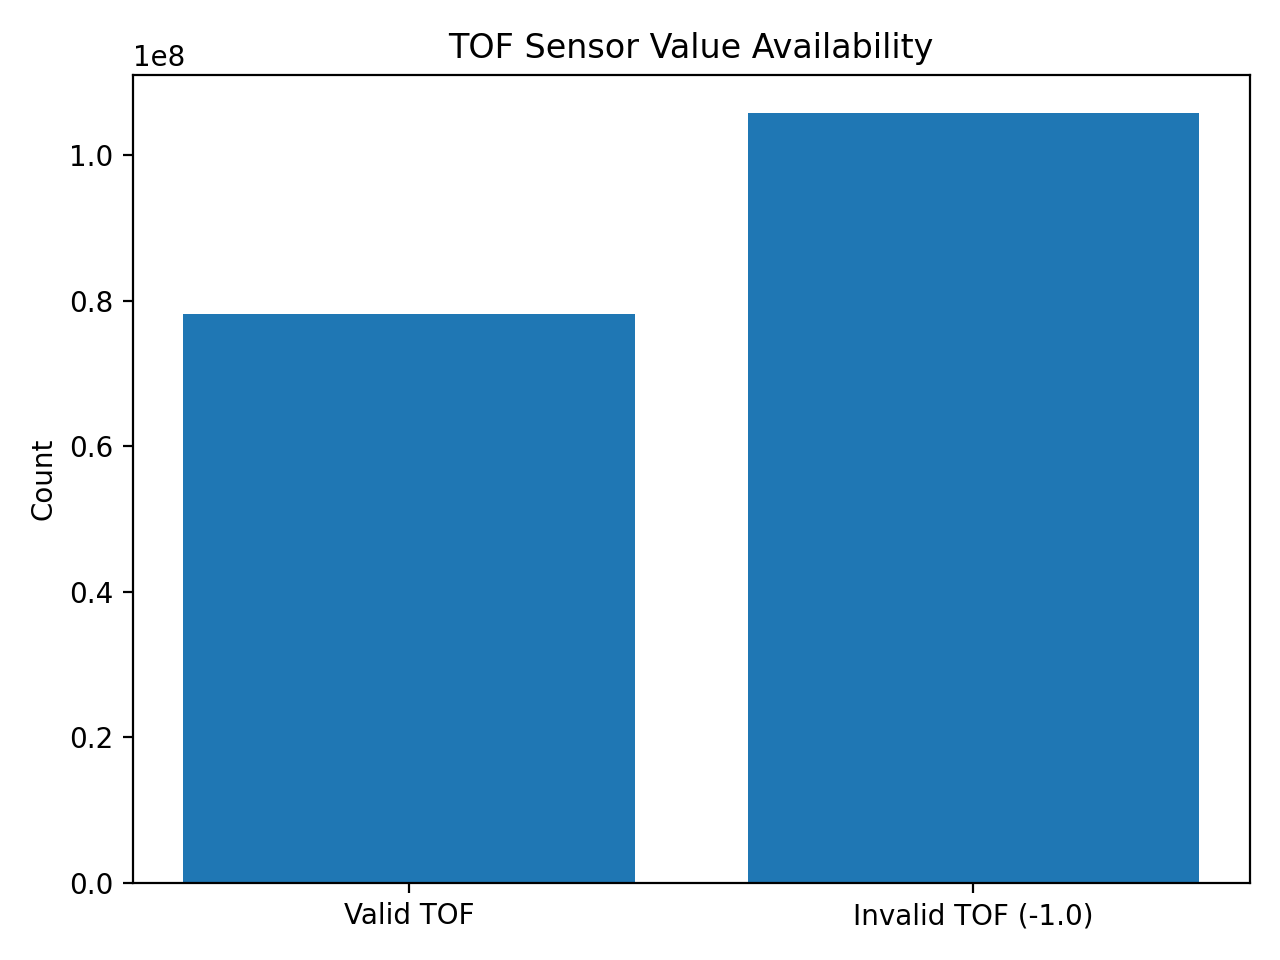
\includegraphics[width=\columnwidth]{plots/tof_invalid_rate.png}
    \caption{Rate of invalid (NULL) sensor readings per TOF channel across the CMI Helios dataset. Approximately 6.7\% of rows contain NULL values. Peripheral TOF channels exhibit higher invalidity rates, motivating their exclusion from the NLP tokenization pipeline.}
    \label{fig:tof}
\end{figure}
 
\subsection{Summary of Results}

The key finding of this evaluation is that NLP-based tokenization of sensor data produces a representation tha improves multi-class gesture discrimination. While the binary BFRB detection task is relatively well solved by both the baseline deep learning models and the NLP models (all achieving above 89\% binary F1), the macro-averaged multi-class task reveals a substantial advantage for the NLP approach. The Transformer model's macro F1 of 85.98\% represents a 35.84 percentage point improvement over the best baseline model (Late Fusion, 50.14\%), demonstrating that treating sensor readings as a structured symbolic language provides better representational basis for distinguishing fine-grained gesture categories.

\vspace{-0.23cm}
 \begin{table}[!ht]
\caption{Summary of Binary and Macro F1 Scores}
\centering
\begin{tabular}{lcc}
\hline
Model & Binary F1 (\%) & Macro F1 (\%) \\
\hline
FFT-MLP (All) & 90.93 & 46.12 \\
FFT-MLP (IMU+THM) & 90.86 & 41.07 \\
CNN-BiLSTM (TOF) & 91.60 & 29.50 \\
Late Fusion & 94.28 & 50.14 \\
Intermediate Fusion & 91.11 & 39.61 \\
Random Forest & 89.81 & 38.80 \\
Transformer (NLP) & 90.93 & 85.98 \\
BiLSTM (NLP) & 89.98 & 84.19 \\
\hline
\end{tabular}
\end{table}

From a model complexity perspective, the Transformer classifier contains 
69,506 parameters while the BiLSTM contains 596,866 parameters a 
difference of approximately 8.6$\times$. Despite this large gap in 
parameter count, the Transformer achieves only 1.79 percentage points 
higher macro F1, suggesting that the self-attention mechanism is 
significantly more parameter-efficient for this tokenized sensor 
classification task. Both models were trained on CPU without GPU 
acceleration, making the Transformer's smaller footprint an additional 
practical advantage for deployment on resource-constrained wearable systems.


\clearpage

















\clearpage
\section{Discussion}
\label{sec:discussion}

The results of this project show a clear difference between binary detection and fine-grained multi-class recognition. On the binary task, the Late Fusion baseline remained the strongest model, reaching a binary F1-score of 93.95\%, while the Transformer and BiLSTM achieved 90.93\% and 89.98\%, respectively. This suggests that the baseline multimodal fusion strategy remains highly effective for separating BFRB gestures from non-BFRB gestures, which is consistent with the reference paper's emphasis on combining complementary sensor modalities for robust detection \cite{zhang2025detection}. From a practical perspective, this is important because reliable binary detection is the first requirement for any wearable monitoring system that aims to support early intervention.

However, the comparison changes substantially when macro-averaged F1-score is considered. The Transformer achieved a macro F1-score of 85.98\% and the BiLSTM achieved 84.19\%, both much higher than the best reproduced baseline score of 50.95\% from Late Fusion. Since macro F1 gives equal importance to each class, this result suggests that the proposed token-based representation is especially helpful for distinguishing among similar gesture categories rather than only detecting whether a target behavior is present \cite{zhang2025detection}. In other words, the reproduced baseline models were still stronger for deciding whether a sequence belongs to the broad BFRB group, but the NLP-based models were much stronger for separating one gesture type from another. This distinction matters because a clinically useful system may eventually need to do more than simply raise a warning. It may also need to identify which type of behavior is being performed in order to support more targeted feedback or intervention.

One possible reason for this improvement is the structure of the NLP pipeline itself. By discretizing selected IMU and thermopile channels into ordered symbolic tokens, the model no longer receives only raw continuous values. Instead, it receives a structured sequence that may make repeated gesture patterns easier to learn. This idea is aligned with the general motivation behind applying NLP methods to sequential data, where ordered token relationships can capture useful long-range context \cite{vaswani2017attention, hochreiter1997lstm}. In this project, such a representation appears to be especially useful for gestures that are similar in broad movement pattern but differ in smaller temporal or sensor-level details. For example, two gestures may both involve hand movement toward the head, but they may differ in timing, thermal pattern, or the order in which sensor states appear. A token-based representation can make such local and sequential differences more explicit to the model.

Another useful point is that the macro F1 improvement was not small. The gap between the Transformer and the best reproduced baseline was more than thirty percentage points. That size of difference suggests that the gain is not only a minor optimization effect. Instead, it points to a meaningful change in how the data is being represented and learned. This strengthens the argument that representation choice is just as important as model choice in this problem. The results suggest that, for multi-class BFRB recognition, the way the sensor sequence is encoded may have a major influence on the final performance \cite{zhang2025detection}. This is an important finding because it shows that improving classification does not always require only larger models or more complex architectures. In some cases, changing the input representation can produce a much larger improvement than changing the classifier alone.

The Transformer performed slightly better than the BiLSTM on both binary and macro F1-score, while also using far fewer parameters. In our experiments, the Transformer had 69,506 parameters, compared with 596,866 for the BiLSTM. A likely explanation is that self-attention can relate distant parts of a token sequence more directly, whereas recurrent models process information step by step through hidden states \cite{vaswani2017attention, hochreiter1997lstm}. Even though the performance gap was not very large, the Transformer's better parameter efficiency is still an important practical result for future model development. A smaller and more efficient model may be easier to train, easier to tune, and more realistic for future deployment in constrained environments. This does not mean that BiLSTM is ineffective. In fact, the BiLSTM still performed strongly and remained close to the Transformer. Instead, the results suggest that both architectures are suitable for the tokenized representation, but the Transformer may offer a better balance between performance and efficiency.

At the same time, the current NLP approach still has important limitations. First, TOF data was excluded from tokenization because of its high dimensionality and irregular invalid readings, even though the reference paper shows that TOF proximity information is highly useful for BFRB detection \cite{zhang2025detection}. This means that the NLP models were not yet tested on the full multimodal sensor setting in tokenized form. Second, the tokenization strategy was based on simple quantile bins, which may remove part of the detailed numerical information contained in the original sensor values. While discretization helps create a stable symbolic sequence, it may also reduce subtle variations that could still carry useful information. Third, all training was performed on CPU, which limited the scale of tuning and the number of experiments that could be explored. These limitations suggest that the current results should be viewed as strong early evidence rather than a fully optimized final system.

There are also broader interpretation limits that should be acknowledged. The reproduced baseline results and the proposed NLP results were both obtained under the specific preprocessing and experimental settings used in this project. Small changes in truncation length, training epochs, token vocabulary design, or selected sensor channels may affect the final scores. In addition, the current discussion is based mainly on evaluation metrics rather than on deeper error analysis across each individual gesture class. More detailed class-level analysis may reveal which gesture categories benefit most from tokenization and which remain difficult even for the NLP models. This would be valuable for understanding whether the remaining errors come from class overlap, sensor limitations, or modeling choices.

\section{Conclusion}
\label{sec:conclusion}

This project investigated whether NLP-based sequence models could be applied to multimodal BFRB gesture detection by converting selected sensor readings into discrete tokens. The results show that this approach is effective for wearable sensor classification, especially for fine-grained multi-class recognition \cite{zhang2025detection, vaswani2017attention, hochreiter1997lstm}. Among the two proposed NLP models, the Transformer achieved the best overall performance, with a binary F1-score of 90.93\% and a macro-averaged F1-score of 85.98\%, while the BiLSTM also performed strongly, reaching 89.98\% binary F1 and 84.19\% macro F1 \cite{vaswani2017attention, hochreiter1997lstm}. Although the NLP models did not exceed the best binary F1-score of the reproduced Late Fusion baseline at 93.95\%, they performed much better on macro-averaged F1-score than all reproduced baselines, including Late Fusion at 50.95\%, which suggests that tokenized sensor representations may help capture gesture-specific differences more clearly than standard continuous-input approaches \cite{zhang2025detection}. Overall, these findings support NLP-style modeling as a promising direction for BFRB detection using wearable sensor data, particularly when detailed gesture-level classification is important, and they suggest that future work combining stronger tokenization methods with richer multimodal inputs may further improve performance \cite{zhang2025detection, vaswani2017attention}. 
\clearpage
\appendices
\section{Appendix}
\label{sec:appendix}

This appendix provides supplementary material that supports the main experimental results. It includes the software environment used for the experiments, the reproduced baseline model results, and the final full model comparison across baseline and NLP-based models.

\begin{figure}[!htbp]
    \centering
    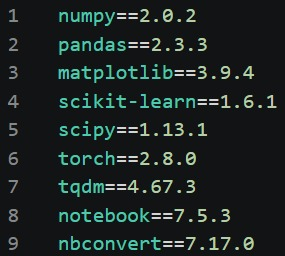
\includegraphics[width=\columnwidth]{Package_List.jpeg}
    \caption{Python package versions used in the experimental environment. These libraries were used for data processing, visualization, notebook execution, and model training.}
    \label{fig:appendix_requirements}
\end{figure}

\begin{figure}[!htbp]
    \centering
    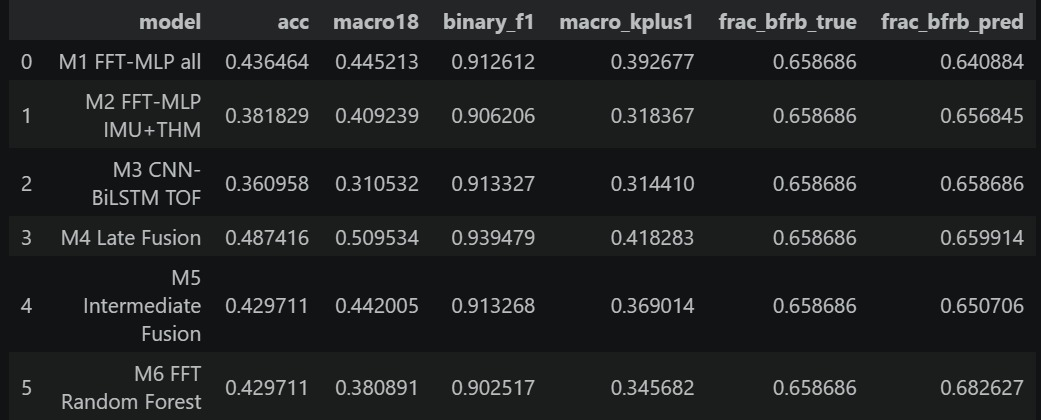
\includegraphics[width=\columnwidth]{evaluation_Table.jpeg}
    \caption{Reproduced baseline model results, including accuracy, macro F1-score, binary F1-score, macro\_kplus1, and predicted BFRB fraction. These results show that Late Fusion achieved the strongest binary classification performance among the reproduced baseline models.}
    \label{fig:appendix_baseline_results}
\end{figure}

\begin{figure}[!htbp]
    \centering
    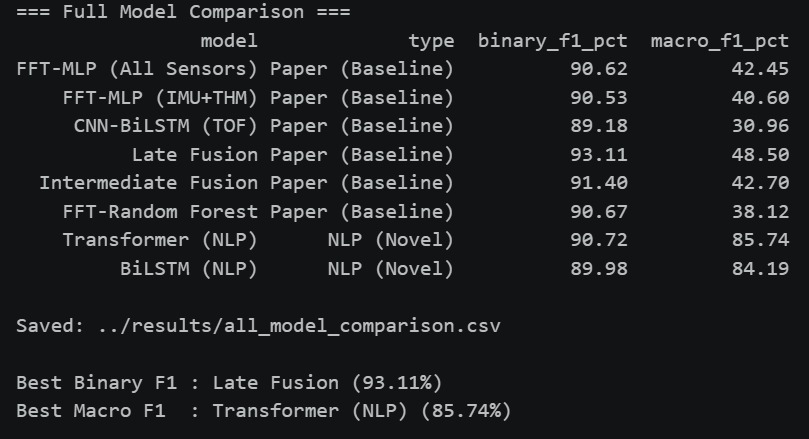
\includegraphics[width=\columnwidth]{Evaluation_Comparsion_Table.jpeg}
    \caption{Full model comparison between reproduced baseline models and the proposed NLP-based models. The Transformer achieved the best macro F1-score, while Late Fusion achieved the best binary F1-score.}
    \label{fig:appendix_full_comparison}
\end{figure}

\clearpage
\bibliographystyle{IEEEtran}
\bibliography{references}

\end{document}
\appendices

\section{Tokenization Example}
\label{sec:appendix_tokenization}

The NLP-based models used in this project rely on a tokenization process that converts continuous sensor readings into discrete symbolic representations. This was done by selecting 12 sensor channels, including 7 IMU channels and 5 thermopile channels, and dividing each channel into three value ranges based on quantile thresholds computed from the training data. These ranges correspond to low, medium, and high signal levels.

For example, if one timestep contains a low value for \texttt{acc\_x}, a medium value for \texttt{rot\_y}, and a high value for \texttt{thm\_3}, the resulting tokens may be written as \texttt{acc\_x\_low}, \texttt{rot\_y\_medium}, and \texttt{thm\_3\_high}. After this step, each gesture sequence is transformed into an ordered list of tokens. This representation allows the models to process sensor data in a language-like format rather than as raw continuous values.

\section{Additional Implementation Notes}
\label{sec:appendix_implementation}

The Transformer and BiLSTM models were both trained on CPU without GPU acceleration. The Transformer used an embedding dimension of 64, two encoder layers, four attention heads, and a feed-forward dimension of 128. The BiLSTM used the same embedding size and two bidirectional recurrent layers with a hidden size of 128 per direction.

Both models used padding-aware sequence handling so that padded values would not influence the final sequence representation. Mean pooling over valid timesteps was applied before the final classification layer. This design allowed both models to generate a fixed-length representation from variable-length gesture sequences.

\begin{table}[!htbp]
\caption{Parameter Counts of NLP Models}
\label{tab:appendix_params}
\centering
\begin{tabular}{lc}
\hline
\textbf{Model} & \textbf{Parameter Count} \\
\hline
Transformer & 69,506 \\
BiLSTM & 596,866 \\
\hline
\end{tabular}
\end{table}

\section{Reproducibility Notes}
\label{sec:appendix_reproducibility}

Several steps were taken to support reproducibility. First, the train-test split was performed at the sequence level to reduce the risk of data leakage. Second, tokenization thresholds were computed using only the training partition and then applied to the test partition. Third, preprocessing, model training, and evaluation were organized as separate stages in the project workflow.

This design makes it easier to rerun the experiments and verify the reported results. It also supports future extensions, such as testing alternative tokenization methods, adding sensor channels, or comparing other sequence modeling architectures.
\clearpage
\bibliographystyle{IEEEtran}
\bibliography{references}

\end{document}
